\documentclass{standalone}
\usepackage{tikz}
\usepackage{amsmath,amsfonts,amssymb}
\usetikzlibrary{automata,positioning}
\begin{document}
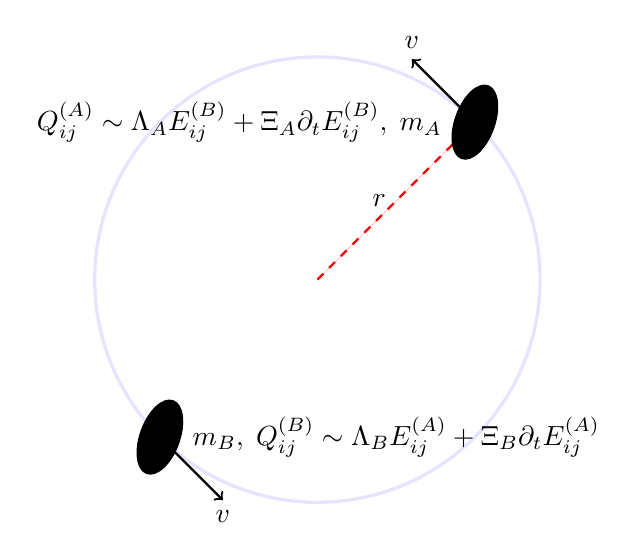
\begin{tikzpicture}
    \draw[color=blue!10, very thick](0,0) circle (2.828);
    \filldraw[red, dashed, thick] ( 0, 0) -- (2, 2) node[midway,left] {\textcolor{black}{$r$}}; 
    \filldraw[rotate around={70:(2,2)},black] (2,2) ellipse (14pt and 7.14pt) node[left] 
	{ $Q^{(A)}_{ij}\sim\Lambda_A E^{(B)}_{ij} + \Xi_A \partial_tE^{(B)}_{ij},\;m_A\;\;\;$};
    \draw[thick, ->] ( 2, 2) -- ( 1.2, 2.8) node[above] {$v$};
    \filldraw[rotate around={70:(-2,-2)},black] (-2,-2) ellipse (14pt and 7.14pt) node[right] 
	{ $\;\;\;m_B,\;Q^{(B)}_{ij}\sim\Lambda_BE^{(A)}_{ij} + \Xi_B \partial_t E^{(A)}_{ij}$};
    \draw[thick, ->] (-2,-2) -- (-1.2,-2.8) node[below] {$v$};
    \end{tikzpicture}
\end{document}


